\section{Durchführung}
\label{sec:Durchführung}

Für die Bestimmung des Schubmoduls $G$ nach der dynamischen Methode wird die in Abbildung \ref{fig:Aufbau} abgebildete
Versuchsapparatur verwendet. 

\begin{figure}
  \centering
  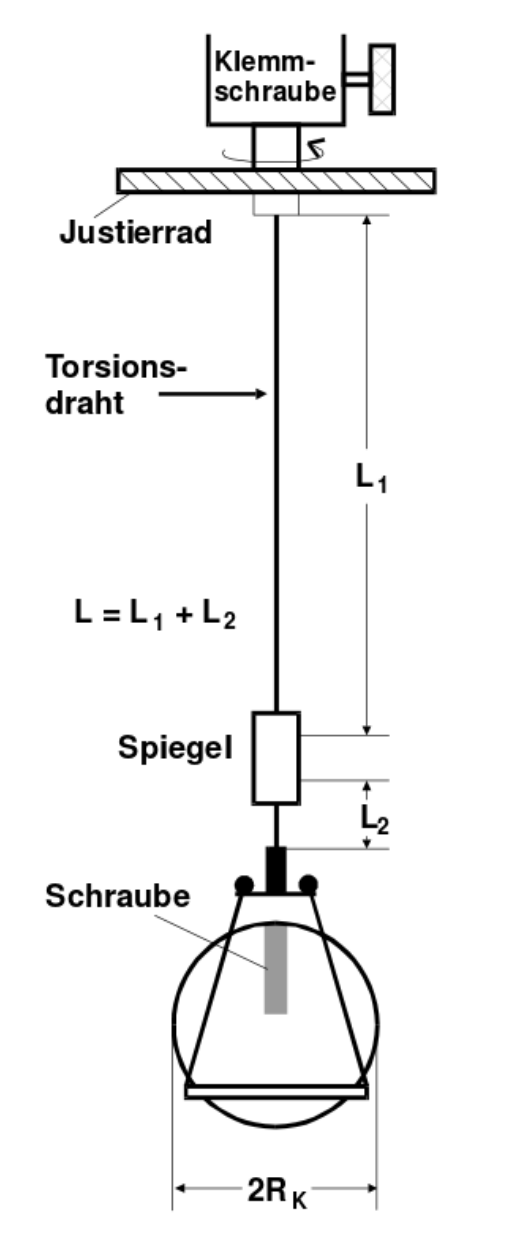
\includegraphics[scale=0.2]{content/Aufbau.png}
  \caption{Messapparatur zur Bestimmung des Schubmoduls eines Torsionsdrahtes. [1]}
  \label{fig:Aufbau}
\end{figure}

In dieser ist eine Kugel an einem Torsionsdraht aufgehängt. Der Draht soll durch eine Auslenkung
mit dem Justierrad zum Schwingen gebracht werden. Für die Unterbindung andersförmiger Bewegungen, 
ist eine Vorrichtung angebracht, mit der die Kugel durch eine Dämpfung in Ruhe versetzt werden 
kann.

Zur Messung der Periodendauer wird nach Abbildung \ref{fig:Licht} ein Lichtstrahl emittiert, 
der durch einen Doppelspalt und eine Sammellinse auf einen am Draht befestigten Spiegel fällt. 
Der Spiegel dreht sich somit zusammen mit der Kugel und dem reflektierten Lichtstrahl, 
welcher an einem Punkt auf eine Fotodiode trifft.

\begin{figure}
  \centering
  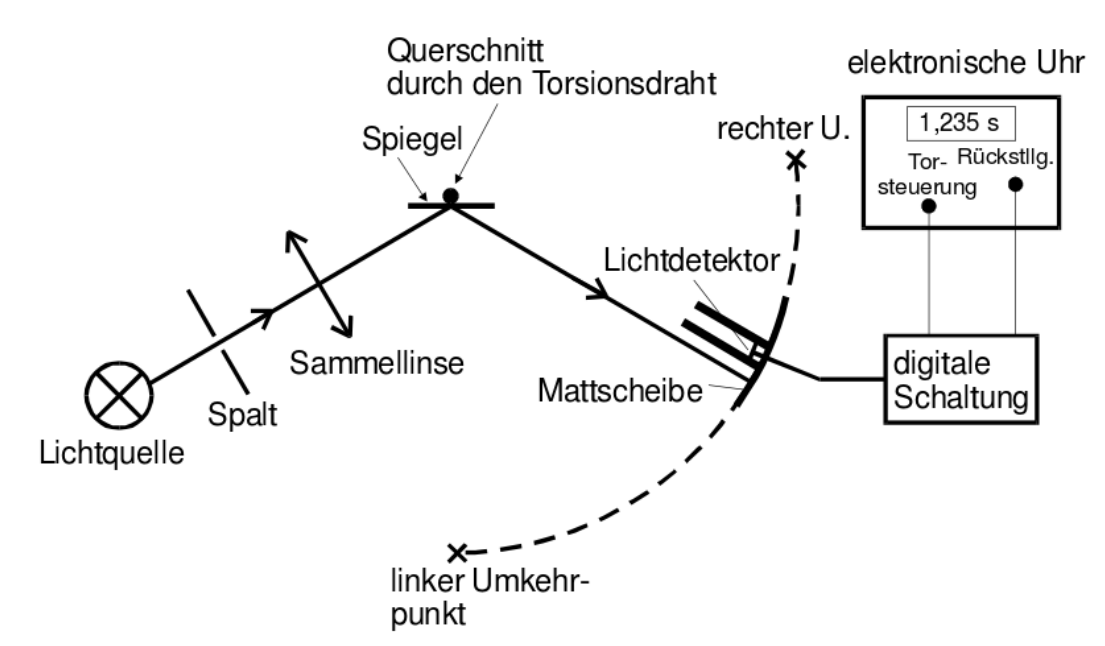
\includegraphics[scale=0.2]{content/Licht.png}
  \caption{Bestimmung der Periodendauer T der Schwingung des Torsionsdrahtes mithilfe eines Lichtdetektors. [1]}
  \label{fig:Licht}
\end{figure}

Das elektrische Signal wird dabei zur Zeitmessung genutzt. Das erste Signal beginnt die Messung,
das zweite muss für eine volle Periode ignoriert werden, was durch eine sogenannte Flip-Flop-Kippstufe realisiert wird.
Das dritte Signal beendet dann die Messung und das vierte setzt die Zähluhr zurück. 
Zu Anfang soll dazu der Draht mittels des Justierrades so justiert werden, dass der Lichtstrahl
auf die, die Diode umgebende, Mattscheibe fällt. Auch sollen die Abstände innerhalb der Beleuchtungsapparatur 
so variiert werden, dass das Beugungsbild möglichst scharf auf der Mattscheibe abgebildet wird.\\

Zusätzlich wird eine Messung zur Bestimmung des magnetischen Dipolmoments $\vec{m}$ eines Permanentmagneten
durchgeführt. Während bei der Messung des Schubmoduls $G$ die Dipolachse der Kugel anhand einer Markierung
parallel zum Draht ausgerichtet werden sollte, um den Einfluss des Erdmagnetfeldes aufzuheben, wird
dieses hier senkrecht zum Draht ausgerichtet. Außerdem wird um den Magneten durch ein Helmholtzspulenpaar
ein homogenes Magnetfeld aufgebaut. Wieder wird die Periodendauer gemessen, diesmal jeweils für verschiedene
magnetische Flussdichten. Außerdem darf der Schwingungswinkel bei dieser Messung nur klein sein, da somit eine 
vereinfachende Winkelnäherung in der Herleitung verwendet werden kann.\\

Außerdem wird mit einer Mikrometerschraube der Durchmesser und mit einem Maßband die Länge 
des Drahtes gemessen. 

